% Team layout
% Budget
%
\begin{wrapfigure}{r}{.4\linewidth}
    \vspace{-2em}
    \centering
    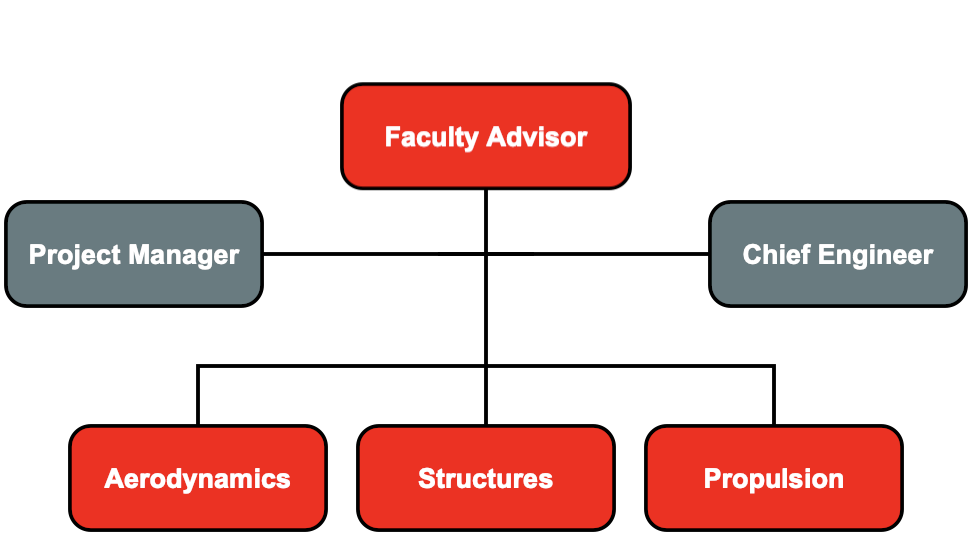
\includegraphics[width=\linewidth]{Images/ts.png}
    \caption{Illinois Tech's team structure.}
    \label{fig:teamstruc}
    \vspace{0.3em}
\end{wrapfigure}
%
IIT's team is student run and has a faculty advisor present to provide necessary guidance. The team is composed of multiple sub-teams that are each responsible for a major design component of the aircraft. Table \ref{tab:teams} describes the roles and skills utilized by each sub-team. A sub-team is led by a team lead who reports to the Project Manager and Lead Engineer (see Figure \ref{fig:teamstruc}). The Lead Engineer oversees all components of the design and ensures cohesion between all sub-team decisions. The Lead Engineer also reports progress and design decisions to the Project Manager. The Project Manager is responsible for ensuring the design progress stays on track, deadlines are being met, and team leads are focusing resources on appropriate tasks.
%
\vfill
\begin{atb}{Description and skills utilized and learned for each sub-team.}{tab:teams}{m{.135\linewidth} >{\raggedright\arraybackslash}m{.42\linewidth} m{.365\linewidth}}
    % Headers
    \makebox[\linewidth]{\centering Sub-team} & 
    \makebox[\linewidth]{\centering\color{white}Responsibilities} &
    \makebox[\linewidth]{\centering\color{white}Associated Skills} \\
    % 
    % Aero
    Aerodynamics
    & Design of lifting bodies, aircraft sizing, aerodynamic performance, and stability analysis.
    & \tabitem Aerodynamics and flight mechanics\par\tabitem XFLR5 and related CFD software \\%\clineB{2-3}{2}
    %
    % Propulsion
    Propulsion
    & \cellcolor{gray!25}Selection of motor/battery combination, setup of remote control systems, and flight data analysis.
    & \cellcolor{gray!25}\tabitem Propulsion sizing tools \par\tabitem Electrical design\par\tabitem System analysis and feedback control \\%\clineB{2-3}{2}
    %
    % Structures
    Structures
    & Design of aircraft structures, mechanical systems, and shipping container along with material selection.
    & \tabitem Structural mechanics\par\tabitem SolidWorks and FEA software\\

\end{atb}
%
    \vspace{1em}
\begin{figure}[H]
    \centering
    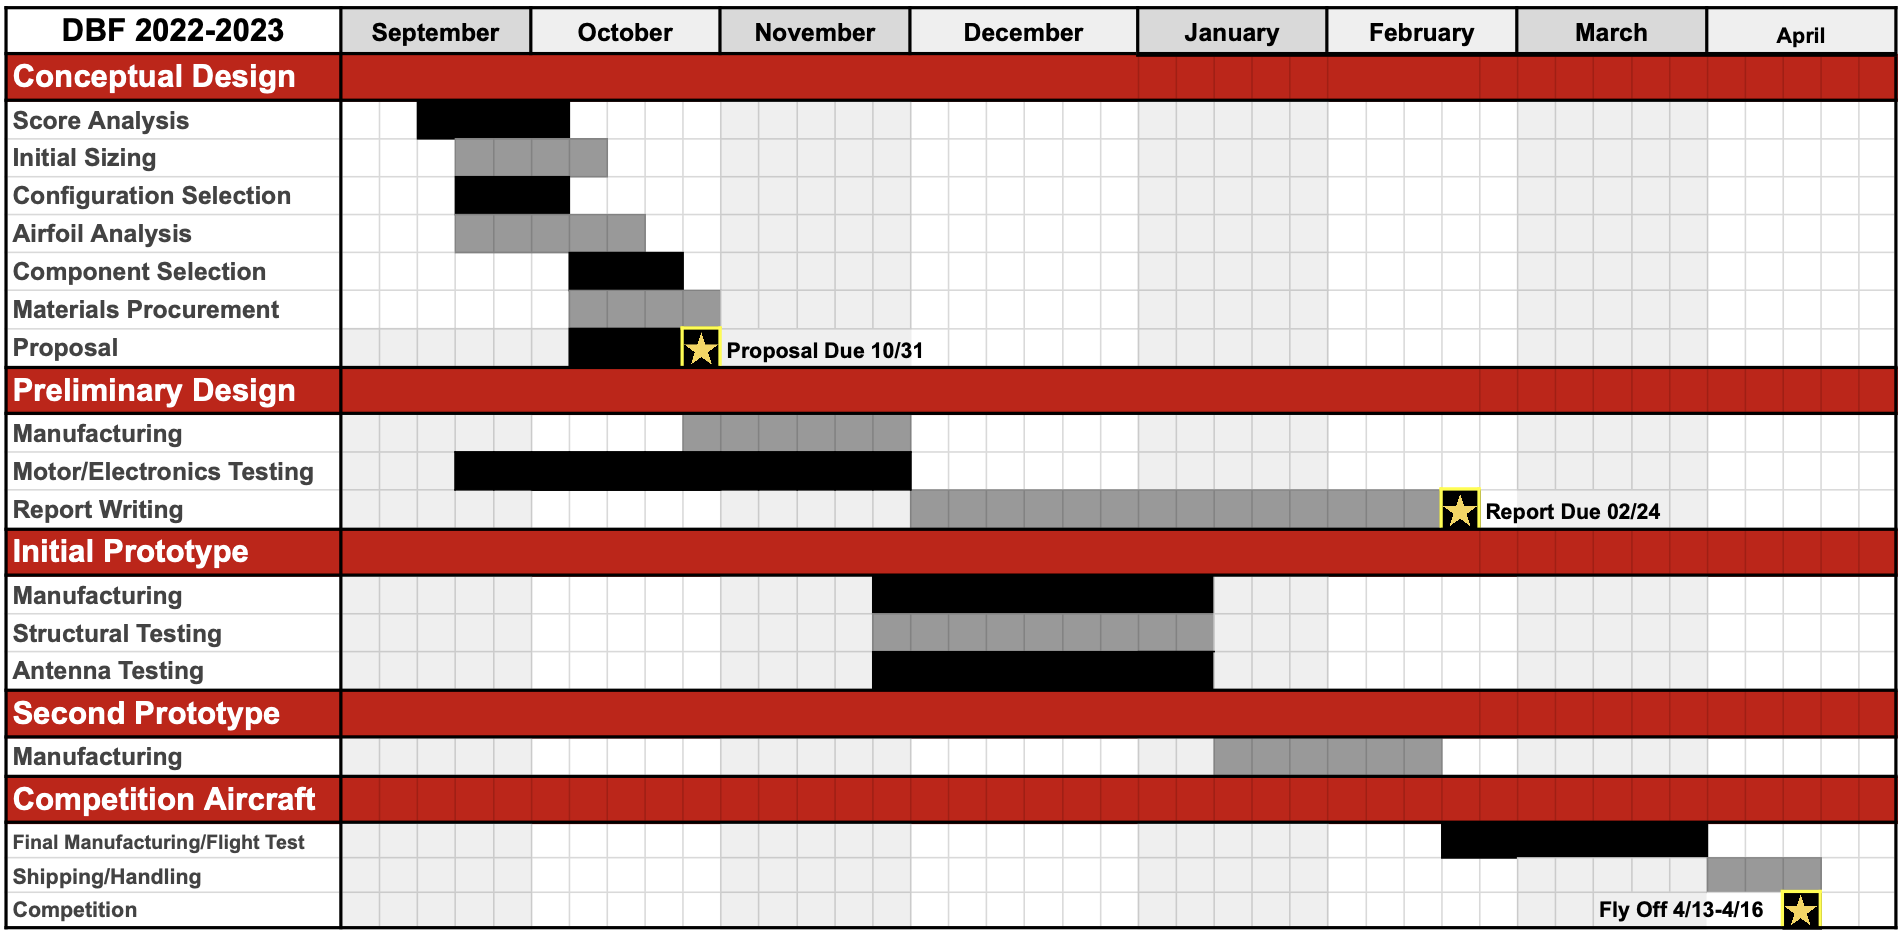
\includegraphics[width=\linewidth]{Images/DBF 22-23 Gantt.png}
    \vspace{-15pt}
    \caption{Illinois Tech Team Milestone Chart}
    \label{fig:gchart}
    \vspace{-.5em}
\end{figure}

A Gantt chart, as shown in Figure \ref{fig:gchart}, is maintained by the Project Manager to monitor project status and distribute resources accordingly. The schedule serves to determine task completion times, delays, and appropriate task order.
% Budget
\subsection{Budget}
    The project will be funded by the Illinois Institute of Technology Student Activity Fund (IIT-SAF) and from individual members of the team. IIT-SAF will fund the entirety of materials and components for testing, design, and approximately 70\% of the costs associated with travel to the competition. A summary of the expected expenses are shown in Table \ref{tab:budget}. The necessary machines and tools are available in IIT's Idea Shop and the AIAA-IIT lab which has been furnished by IIT-SAF.
    % The expected cost per student traveling to contest is \$95.
  
    % {\renewcommand{\arraystretch}{1}
    % \begin{atb}{Proposed Budget with Funding Sources}{tab:budget}{m{1.25in} >{\raggedright\arraybackslash}m{.5\linewidth} >{\raggedleft\arraybackslash}p{.075\linewidth} m{.17\linewidth} m{.365\linewidth}}
    %     Item & \mc{1}{c}{\color{white}Description} & \mc{1}{c}{\color{white}Cost} & \mc{1}{c}{\color{white}Fund Source} \\
    %     %
    %     Structural materials
    %     & Balsa, plywood, adhesives, hardware
    %     & \$1120
    %     & 100\% IIT-SAF \\
    %     %
    %     Propulsion system
    %     & \cellcolor{gray!25}Motors, ESC, battery, propellers
    %     & \cellcolor{gray!25}\$385
    %     & \cellcolor{gray!25}100\% IIT-SAF \\
    %     %
    %     Control system
    %     & Wiring, servos, RC controller, receiver
    %     & \$130
    %     & 100\% IIT-SAF \\
    %     %
    %     Miscellaneous
    %     & \cellcolor{gray!25}Landing gear, monokote, tools
    %     & \cellcolor{gray!25}\$225
    %     & \cellcolor{gray!25}100\% IIT-SAF \\
    %     %
    %     Hotel
    %     & 3 rooms for 4 nights
    %     & \$1550
    %     & 30\% Self Funded. 70\% IIT-SAF \\
    %     %
    %     Transportation
    %     & \cellcolor{gray!25}Airfare for 7, 2 cars for 5 days + gas 
    %     & \cellcolor{gray!25}\$5500
    %     & \cellcolor{gray!25} 30\% Self. 70\% IIT-SAF\\ \hlineB{2.5}
    %     %
    %     Total & & \$8910 & 
    % \end{atb}}

    {\rowcolors{10}{gray!10}{white}
        \begin{atb}{Proposed Budget with Funding Sources}{tab:budget}{l *{6}{c|}}
            \makebox[.2\linewidth]{\centering Expenses} & \color{white}Description & \color{white}Cost & \color{white}Funding Source\\
        Structural materials 
        & Balsa, plywood, adhesives, hardware
        & \$1120
        & 100\% IIT-SAF \\
        %
        Propulsion system
        & \cellcolor{gray!25}Motors, ESC, battery, propellers
        & \cellcolor{gray!25}\$385
        & \cellcolor{gray!25}100\% IIT-SAF \\
        %
        Control system
        & Wiring, servos, RC controller, receiver
        & \$130
        & 100\% IIT-SAF \\
        %
        Miscellaneous
        & \cellcolor{gray!25}Landing gear, monokote, tools
        & \cellcolor{gray!25}\$225
        & \cellcolor{gray!25}100\% IIT-SAF \\
        %
        Air Travel
        & 7 Students, \$450 per person 
        & \$3150
        & 30\% Self. 70\% IIT-SAF \\
        %
        Hotel
        & \cellcolor{gray!25}3 rooms for 4 nights
        & \cellcolor{gray!25}\$1800
        &\cellcolor{gray!25} 30\% Self. 70\% IIT-SAF \\
        %
        Transportation
        & 2 Cars for 5 days + gas 
        & \$1500
        & 30\% Self. 70\% IIT-SAF\\ \hlineB{2.5}
        %
        Total & & $\bold{\$8310}$ & \\ \hlineB{2.5}
        \end{atb}}